\documentclass[12pt]{amsart}
\usepackage{amsmath, amssymb, amsthm}
\usepackage[margin=2.5cm]{geometry}
\usepackage{hyperref}
\usepackage{booktabs}
\usepackage{graphicx}

\newtheorem{observation}{Observation}
\newtheorem{derivation}[observation]{Derivation}
\newtheorem{remark}[observation]{Remark}

\title[The Riemann zero lattice as a warm crystal]{The Riemann zero
lattice as a warm crystal:\\ diffraction, screening, and the two-branch
response}

\author{U\u{g}ur Sezen}
\address{Independent researcher, Istanbul, Turkey}
\email{ugursezen@gmail.com}

\date{\today}

\begin{document}

\begin{abstract}
Three companion notes measured how the local statistics of Riemann zeros
respond to the prime waves of the explicit formula, and identified a
sampling-grid systematic: the gap midpoints on which all such
measurements stand are themselves displaced by the primes. Here we turn
the grid into the object. Its structure factor
$\hat G(\omega) = \langle e^{i\omega t_n}\rangle$ --- the diffraction
pattern of the zero lattice --- decomposes into three measured
components: \emph{arithmetic spots} at $\omega = \log p^k$,
\emph{Bragg combs} damped by the lattice temperature, and a
\emph{dark field} lying a factor $\sim 25$ below shot noise
(hyperuniformity seen directly in diffraction). The spots obey an
absolute, parameter-free law derived from the explicit formula,
$|\hat G(\log q)| = \Lambda(q)\,(L\sqrt{q})^{-1}\cos(\pi\tau)
\cdot \mathrm{DW}$, verified to $0.1$--$4\%$ across fifteen prime and
prime-power lines, with phases pure real to $0.6^\circ$; the comb
brightness tracks the measured window temperature ($e^{-c}$, ratio
$0.885$ constant across windows, most of the deviation from Gaussian
explained by the measured negative excess kurtosis); and binned over
the spots, the pattern rebuilds the Montgomery ramp in the first
line-bearing bin --- Berry's semiclassical decomposition observed
directly. The grid systematic of the companion revisions closes into an
identity: all Gram couplings between wave columns are values of
$\hat G$, and the regression-dressing lives in the thermal diffuse
scattering between the dark field and the comb. On the gap side, the
same displacement field yields a derived sum rule for the
zero-displacement channel --- onset $v = 2\tau$ and saturation scale
$2/\pi$ --- with $\Lambda$-weighting confirmed for prime powers
($k \cdot v(p^k)$ lands on the prime curve to $1$--$5\%$); the residual
is a \emph{screening function} $D(\tau)$, isolated by injection
calibration. Finally, the conditional gap response splits into two
branches: to its own spontaneous fluctuations the gas responds exactly
like CUE for $\tau \gtrsim 0.3$ (agreement to $0.5\%$ at the Nyquist
wavevector --- a new CUE test independent of pair-correlation
statistics), while below the first prime line it is frozen
($D \approx 0.04$); the coherent prime branch instead starts near unity
and is screened to $0.48$, the two branches crossing at
$\tau \approx 0.17$. Two candidate mechanisms for the measured
prime-power weight deficit are refuted by a phase-purity test, and the
surviving constraints are stated as open problems.
\end{abstract}

\maketitle

\section{Introduction}

The first three notes of this program \cite{companion1, companion2,
companion3} measured the joint law of consecutive-zero gaps $\delta_n$
and between-zero maxima of Hardy's $Z$, dissected it into explicit-formula
channels --- an amplitude transmission $w(\tau)$ and a zero-displacement
response $v(\tau)$, $\tau = \log p / L$, $L = \log\frac{t}{2\pi}$ ---
and organized the channels into a response theory: a two-channel linear
constraint, a sign crossing at $\tau_0 = 0.447$, a thermal Bragg mirror
at the Riemann--Siegel fold that reproduces it, and a mirror
(functional-equation) interference channel.

The revision of those notes was forced by a discovery about the
\emph{measurement} itself: every per-gap regression stands on the gap
midpoints, and the midpoints are not a passive grid --- the zeros are
displaced by the prime waves, so the grid carries the primes, restricted
regression bases transfer omitted-line content into retained
coefficients, and a ground-truth test showed the transfer reaches
$0.14$--$0.24$ in absolute $w$ units. The companions correct for this by
the complete-basis convention. The present note takes the opposite
attitude: \emph{the bending ruler is not a nuisance --- it is the
cleanest window into the zero lattice that this program has found.}
Throughout, the style of the companions is kept: no closed forms are
fitted; every ingredient is measured or derived; every claim is
accompanied by the test that tried to kill it, and two failed
derivations are reported as such.

Data: the six primary amplitude windows of \cite{companion2}
($4\times10^4$ gaps each, $L = 9.86$ to $12.45$), with the auxiliary
windows of the companions where noted. All measurements are per-window
and pooled; placebo and surrogate controls accompany each new
observable.

\section{The diffraction pattern}\label{sec:diff}

Define the structure factor of the midpoint grid,
\[
\hat G(\omega) \;=\; \frac{1}{n}\sum_{n} e^{i\omega t_n},
\qquad t_n = \text{gap midpoints},
\]
--- operationally, the diffraction pattern of the zero lattice. Three
components appear (Figure~\ref{fig:diff}).

\emph{Arithmetic spots.} At $\omega = \log q$, $q = p^k$, the pattern
shows sharp spots. To first order in the displacement field $u$
(defined by $t_n = t_n^{\mathrm{smooth}} + u_n$),
$\hat G(\omega) \approx i\omega \langle e^{i\omega t^{s}} u\rangle$, so
a $u$-line of amplitude $U_q$ at $\log q$ produces a spot
$|\hat G| = \tfrac{\omega}{2} U_q \cos(\pi\tau)$, the $\cos(\pi\tau)$
being the midpoint-averaging factor over one lattice spacing
(measured independently by injection, below). The spots are
\emph{phase-locked}: across eleven primes, six windows, and eight prime
powers, $\arg \hat G(\log q) = 180.0^\circ$--$180.6^\circ$ with
quadrature parts consistent with zero at the $10^{-4}$ level --- the
displacement field is sine-locked, exactly as a real gap-channel
response demands.

\emph{Bragg comb.} In the unfolded frame the lattice's own reflection
sits at $\omega_x = 2\pi k$. Its first-order brightness is the
characteristic function of the midpoint phase; the Gaussian
(Debye--Waller) estimate $e^{-c}$, with $c = (2\pi\sigma_u)^2/2$ the
measured jitter of the companion notes, overshoots by a constant factor:
measured/Gaussian $= 0.88$--$0.89$ across all six windows. The measured
excess kurtosis of the wrapped midpoint phase ($-0.75$ to $-0.79$)
explains most of the gap through the Edgeworth correction
($0.32 \to 0.27$ vs measured $0.256$ at $L = 9.86$); a $\sim 6\%$
remainder is left to higher cumulants. The second-order comb is
extinguished (measured at the noise floor), as strong dephasing
predicts. The comb brightness thus tracks the window temperature
window-by-window --- a third, independent thermometer for the thermal
Bragg model of \cite{companion3}.

\emph{Dark field.} Off the lines and away from the comb, the pattern is
\emph{dark}: the median $|\hat G|$ over $1200$ off-line frequencies is
$2\times10^{-4}$, a factor $\sim 25$ \emph{below} the shot-noise level
$1/\sqrt{n}$, and below a shuffled-gap surrogate (which destroys the
anticorrelations and raises the floor to $1.4\times10^{-3}$).
Hyperuniformity of the zero gas --- number-variance rigidity --- is here
seen directly as darkness in a diffraction pattern. All arithmetic
content is concentrated in the discrete spots.

\begin{figure}[ht]
\centering
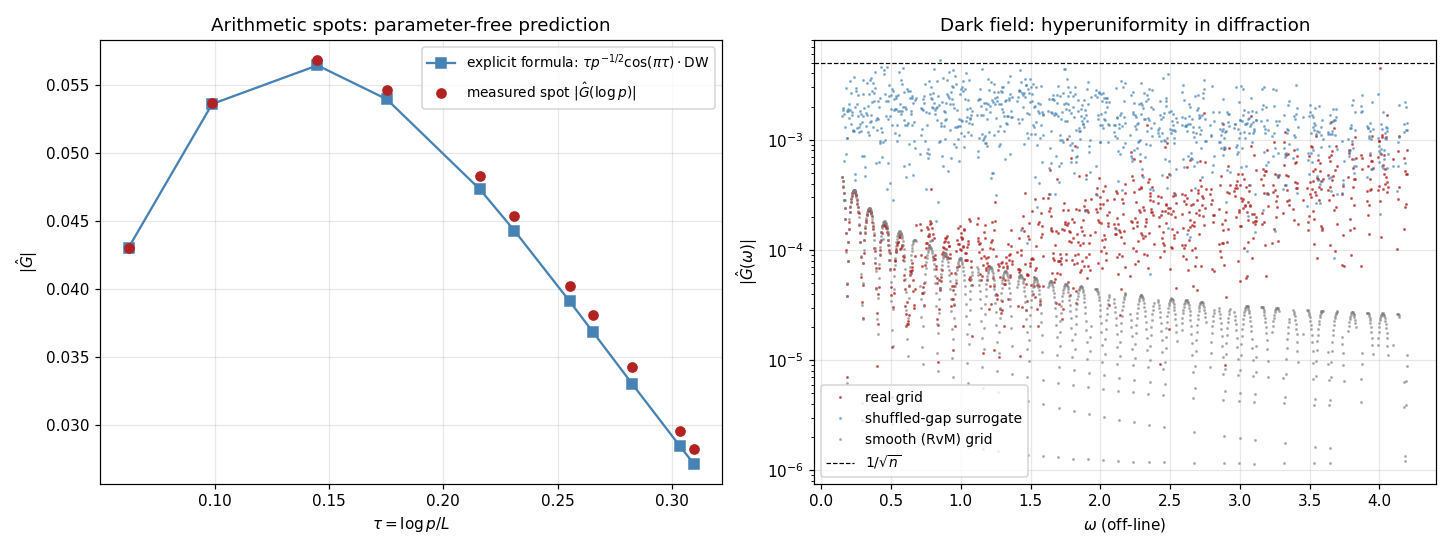
\includegraphics[width=0.95\textwidth]{fig_diffraction_en.png}
\caption{Left: arithmetic spots against the absolute explicit-formula
prediction of Section~\ref{sec:abs}. Right: the off-line dark field for
the real grid, a shuffled-gap surrogate, and the smooth grid; dashed
line is shot noise.}
\label{fig:diff}
\end{figure}

\section{The absolute spot law}\label{sec:abs}

\begin{derivation}
The truncated explicit formula gives the argument function the line
content $S(t) \supset -\tfrac{1}{\pi}\,
\frac{\Lambda(q)}{\sqrt{q}\,\log q}\,\sin(t\log q)$, and the zero
displacement is $u = -S/\bar\rho$ with $\bar\rho = L/2\pi$; hence the
$u$-line amplitude
\[
U_q \;=\; \frac{2\Lambda(q)}{L\sqrt{q}\,\log q},
\]
and the spot law, with no reference to any channel measurement,
\[
|\hat G(\log q)| \;=\; \frac{\Lambda(q)}{L\sqrt{q}}\,
\cos(\pi\tau)\; e^{-\omega^2\sigma_t^2/2}.
\]
\end{derivation}

\begin{observation}[Absolute spot law]
Across the six windows, measured/predicted $= 0.999$ ($p=2$), $1.002$
($p=3$), $1.007$, $1.012$, $1.021$, $1.024$, $1.030$, $1.032$, $1.036$,
$1.039$, $1.040$ ($p=31$); mean $1.022 \pm 0.014$. The prediction has
\emph{no} free parameters and \emph{no} channel input: the explicit
formula predicts the diffraction pattern of the zero lattice at the
percent level. The mild $+2$--$4\%$ rise with $\omega$ is consistent
with the Gaussian DW factor slightly over-damping a sub-Gaussian field
and is left as a second-order refinement.
\end{observation}

For prime powers the same law carries $\Lambda(p^k) = \log p$: the
$1/k$ suppression relative to a $\log q$ weighting. Both channels
confirm it (Section~\ref{sec:gap}); the strong power spots ($q = 4, 8,
9$) obey the absolute law to $1$--$4\%$, while the weak ones fall
progressively below it --- the \emph{power deficit} of
Section~\ref{sec:deficit}.

The spot brightness also closes a loop with the gap channel: the ratio
of the measured spot to the naive $v$-based prediction is a pure
sampling-geometry factor, $\pi\tau\cot(\pi\tau)$ (the gap regression
measures the wave's \emph{difference}, $2\sin(\pi\tau)$, the midpoints
carry its \emph{average}, $\cos(\pi\tau)$), times a constant: measured
ratio$/f(\tau) = 1.083 \pm 0.007$, flat across all eleven primes
(Figure~\ref{fig:geom}). The constant is the inverse of the small-$\tau$
screening $D$ of Section~\ref{sec:gap} ($1/0.92 \approx 1.087$),
closing consistently. Note $f(1/2) = 0$: the vanishing of midpoint
spots at the fold is the sampling Nyquist condition.

\begin{figure}[ht]
\centering
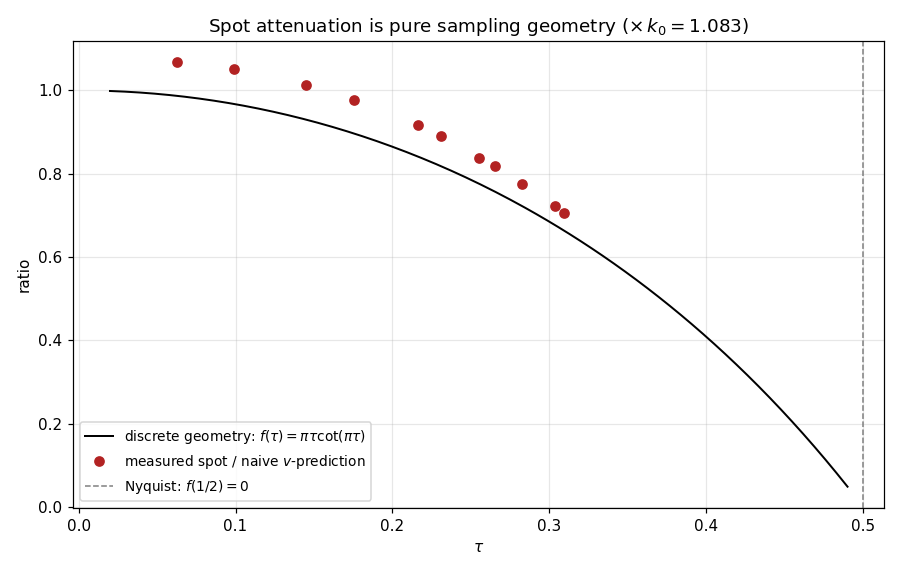
\includegraphics[width=0.62\textwidth]{fig_geometry_en.png}
\caption{Spot attenuation against the naive $v$-based prediction
collapses onto the discrete sampling geometry $\pi\tau\cot(\pi\tau)$,
times the flat constant $k_0 = 1.083 \pm 0.007$.}
\label{fig:geom}
\end{figure}

\section{The ruler identity and the origin of the dressing}

The Gram coupling between any two wave columns on the real grid is an
exact functional of $\hat G$:
\[
\langle \cos(\omega_a t)\cos(\omega_b t)\rangle
= \tfrac12\,\mathrm{Re}\!\left[\hat G(\omega_a - \omega_b)
+ \hat G(\omega_a + \omega_b)\right],
\]
(and the analogous sine combinations), verified numerically to
$5\times10^{-8}$ against directly computed Grams. The omitted-variable
transfer that biased restricted-basis channel measurements
\cite{companion2, companion3} is therefore entirely a property of the
diffraction pattern. Decomposing the transfer line by line shows it is
\emph{collective} --- all eleven omitted small-prime lines contribute
with the same sign, none dominating --- and the carrier frequencies sit
not on arithmetic lines but on the \emph{thermal diffuse scattering}:
the rising flank of $|\hat G|$ between the hyperuniform dark field and
the Bragg comb, at $4$--$15$ times the local dark floor, of the
magnitude a one-dimensional warm crystal predicts
($\sqrt{(1 - e^{-\omega^2\sigma^2})/2n} \approx 3.5\times10^{-3}$ at
$\omega = 6.5$ against measured $5$--$9\times10^{-3}$). In one
sentence: \emph{what bends the regressions is the thermal diffuse
scattering of the zero crystal.}

Binned over frequency, the pattern makes contact with the Montgomery
form factor \cite{Montgomery73}: with $F = n|\hat G|^2$ and
$\alpha = \omega/L$, the sub-first-line region carries
$\bar F = 0.002$ against the ramp value $0.036$ (a factor $18$ dark),
while the first line-bearing bin recovers the ramp from the spots alone
($0.102$ vs $0.089$), with the off-line continuum $10$--$20$ times
below throughout --- Berry's semiclassical construction of the GUE ramp
out of prime lines \cite{Berry88}, observed directly on the midpoint
grid. At larger $\alpha$ the binned means fall behind the ramp in the
same region where the $v$-channel saturates; we record, as a theory
target, that the ramp theorem plus the spot law constitute a sum rule
constraining $v(\tau)$ from first principles.

\section{The gap-channel sum rule and the screening function}
\label{sec:gap}

Carrying the derived $U_q$ through the difference geometry of the gap
channel gives a closed-form prediction,
\[
v(\tau) \;=\; \frac{2}{\pi}\,\sin(\pi\tau)\, ,
\]
which reproduces, with no fitting, the two long-standing empirical
constants of this program: the linear onset $v \approx 2\tau$ (measured
$2.014\,\tau$ under the previous convention) and the saturation scale
$2/\pi = 0.637$ near the fold (measured $0.55$--$0.60$). Against the
$132$ complete-basis measurements the shape holds with a free amplitude
$0.530$ (Figure~\ref{fig:bridge}).

Injection calibration --- adding a synthetic wave of known amplitude to
the \emph{real} zero sequence and passing it through the identical
pipeline --- shows the cosine (midpoint) geometry exact to a few
percent, and the pipeline nearly faithful on the sine side
($a_v = 1.00$--$0.85$ from $\tau = 0.06$ to $0.50$). The residual,
\[
D(\tau) \;=\; \frac{v_{\mathrm{meas}}}{2\tau\, a_v(\tau)}
\;=\; 0.91 \to 0.48 \quad (\tau: 0.05 \to 0.55),
\]
is therefore a physical \emph{screening function}: the gap (difference)
channel responds to the coherent prime drive less than rigid
displacement predicts, while the position (average) channel responds in
full. An additive core --- fluctuations independent of the lines ---
would give $D \equiv 1$; the measurement excludes it. The zeros move
partly \emph{collectively} under the prime waves: translations are
free, compressions are resisted.

\emph{$\Lambda$-weighting and $1/k$.} For prime powers the derived
$v(p^k) = \tfrac{2}{\pi}\sin(\pi\tau)\,D/k$ predicts that
$k\,v(p^k)$ lands on the prime curve. Measured (ratio test,
independent of $D$'s shape): $1.013 \pm 0.009$ ($q=4$),
$1.005 \pm 0.014$ ($8$), $1.005 \pm 0.009$ ($9$), $0.953 \pm 0.021$
($16$), $0.984 \pm 0.012$ ($25$), $0.953 \pm 0.019$ ($27$); the
alternative ($\log q$ weighting, ratio $\approx k$) is excluded. The
$v$-law is a law of $\Lambda$.

\begin{figure}[ht]
\centering
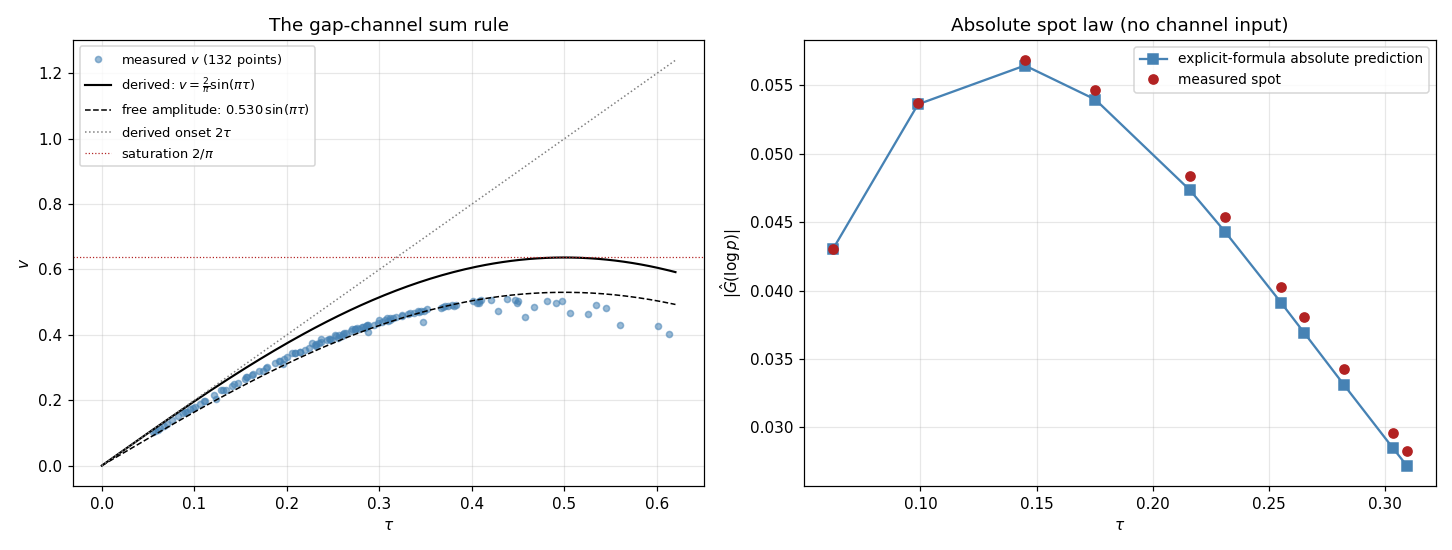
\includegraphics[width=0.95\textwidth]{fig_bridge_en.png}
\caption{Left: the derived gap-channel sum rule against the $132$
complete-basis $v$ measurements. Right: the absolute spot law.}
\label{fig:bridge}
\end{figure}

\section{The two-branch response}\label{sec:branches}

Is the screening a property of the gas or of the drive? Define the
conditional gap response at wavevector $\kappa = 2\pi\tau$: the
regression of gap-content on position-content, normalized so that a
rigid displacement wave gives $1$. Three measurements answer
(Figure~\ref{fig:branch}).

\emph{The CUE reference.} For the circular unitary ensemble the
response is computable without Monte Carlo, by exact
covariance (linear response) over $3000$ sampled spectra, with the
Diaconis--Shahshahani moments \cite{DS94}
($\langle|\mathrm{Tr}\,U^m|^2\rangle = \min(m, N)$) reproduced as an
internal check. CUE does \emph{not} screen: $D_{\mathrm{CUE}} = 1.00 \to
1.18$ from $\kappa \to 0$ to the Nyquist point.

\emph{The spontaneous branch.} The same conditional response measured
on the zeta grid's \emph{own} off-line fluctuation modes (pseudo-ensembles
of $\sim 900$ line-free frequencies per band; local unfolding, cubic
detrending, and phase-scrambled surrogate floors all verified) gives:
\[
D_{\mathrm{spont}} = 0.04\;(\tau{=}0.04),\; 0.24\;(0.06),\;
0.49\;(0.08),\; 0.66\;(0.10),\; 0.93\;(0.15),\; 0.96\;(0.20),
\]
then $1.05$, $1.11$, $1.18$ at $\tau = 0.3$, $0.4$, $0.5$ --- matching
CUE to $0.5\%$ at Nyquist. Two facts stand out. First, for
$\tau \gtrsim 0.3$ the zero gas responds to its own noise
\emph{exactly like CUE}: a new agreement test, independent of
pair-correlation statistics. Second, below the first prime line
($\tau_2 = \log 2/L \approx 0.067$) the gas is \emph{frozen}: position
modulations exist but gaps do not breathe --- the sub-ramp
(quasi-random) regime of the form factor, where the dark field is a
factor $18$ below the GUE ramp, is rigid, and the thaw to CUE behavior
occurs across precisely the band where the first prime lines turn on.

\emph{The prime branch.} The coherent arithmetic drive behaves
oppositely: $D_{\mathrm{prime}}$ \emph{starts} near unity at long
wavelengths (where the spontaneous branch is frozen) and is screened to
$0.48$ at the fold (where the spontaneous branch exceeds unity). The
two branches cross at $\tau \approx 0.17$. The prime waves act as
quasi-static deformations of the equilibrium frame --- followed
adiabatically at long wavelength, resisted at short --- while the
spontaneous long-wave modes are collective translations that carry no
compression. A theory of either branch, and of their crossing scale, is
open.

\begin{figure}[ht]
\centering
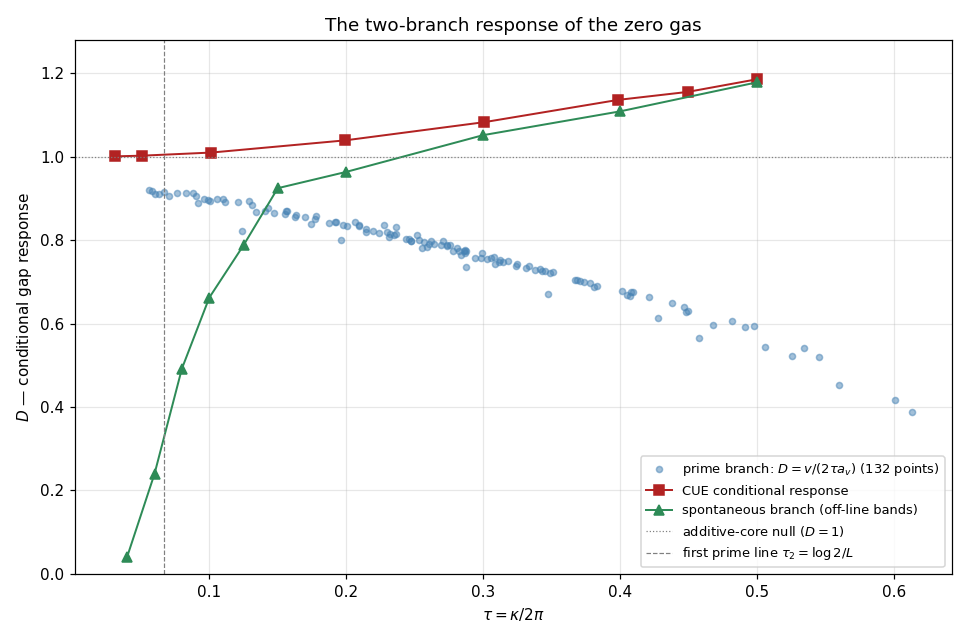
\includegraphics[width=0.7\textwidth]{fig_twobranch_en.png}
\caption{The two-branch conditional gap response: the coherent prime
branch (screened), the spontaneous branch (frozen below the first prime
line, CUE-like above $\tau \approx 0.3$), and the CUE reference.}
\label{fig:branch}
\end{figure}

\section{The power deficit: two failed mechanisms and a constraint
set}\label{sec:deficit}

Prime-power lines carry slightly less than full $\Lambda$ weight, a
deficit growing with $q$ and $k$, seen consistently in three
independent objects (unconditioned channel contents, diffraction spots,
and mildly in the gap-ratio test): spot ratios $0.99$ ($q{=}4$), $0.96$
($8$), $0.98$ ($9$), then $0.87$, $0.89$, $0.81$, $0.65$, $0.72$ for
$q = 16, 25, 27, 32, 49$.

Two mechanisms were built and killed. A noiseless laboratory lattice
obeying the implicit zero condition $\bar\rho\,u = -S(t+u)$ with exact
explicit-formula lines reproduces a power-selective deficit of the
right ordering --- but necessarily rotates the power-spot phases by
$10$--$30^\circ$; the real spots are pure $180^\circ$ to
$0.1$--$0.6^\circ$, so the coherent second-order mechanism is excluded
(the real field's random component decoheres it). A Bessel-type
harmonic-sampling mechanism (power spots fed by the parent prime line
through the sampling exponential) preserves phase but fails
quantitatively ($J_4$ far too small for $q=16$; the $q=49$ vs $q=25$
ordering inverted relative to the parent-line hierarchy).

What survives is a sharp constraint set for the true mechanism: it is
\emph{phase-preserving} (a real multiplicative factor), \emph{selects
prime powers} while leaving primes exact at the $10^{-3}$ level, and
\emph{grows with both $q$ and $k$}. The natural remaining candidate ---
second-order corrections to the $S(t)$ line amplitudes themselves ---
is stated as an open analytic problem.

\section{Synthesis and open problems}

The zero lattice, viewed through its own diffraction pattern, is a warm
one-dimensional crystal: arithmetic spots whose brightnesses the
explicit formula predicts absolutely; a Bragg comb whose brightness is
the window thermometer; thermal diffuse scattering that is precisely
the agent bending every restricted regression; and a hyperuniform dark
field whose binned average rebuilds the Montgomery ramp out of prime
lines. On this substrate the gap channel obeys a derived sum rule
($2\tau$ onset, $2/\pi$ scale) filtered through a measured screening
function, and the conditional response splits into two branches ---
frozen-to-CUE for the gas's own noise, near-unity-to-screened for the
coherent primes --- crossing at $\tau \approx 0.17$.

Open problems: (1) the power-deficit mechanism under the three
constraints of Section~\ref{sec:deficit}; (2) a theory of the screening
function $D(\tau)$ and of the spontaneous branch's freeze-to-CUE
transition, including the crossing scale $\tau \approx 0.17$; (3) the
ramp-plus-spot-law sum rule as a first-principles derivation of the
$v$-normalization and of $k_0$; (4) the $6\%$ non-Edgeworth remainder
of the comb and the sub-Gaussian refinement of the spot DW factor;
(5) the low-$\tau$ frozen regime as a compressibility statement ---
what, precisely, is rigid below the first prime line?; (6) the same
diffraction program for Dirichlet $L$-functions: which spots move,
which constants persist?

\section*{Reproducibility}

All measurements are scripts 79--94 in
\url{https://github.com/azizran/deney} (directory \texttt{qm\_riemann/}),
runnable from the stored datasets; the dated research log records the
two failed mechanisms of Section~\ref{sec:deficit} alongside the
results, together with the audit trail of the companion revisions.

\section*{Acknowledgements}

Computational assistance, literature search and drafting: Claude
(Anthropic). Errors are the author's.

\begin{thebibliography}{9}

\bibitem{Berry88} M.~V.~Berry, \emph{Semiclassical formula for the number
variance of the Riemann zeros}, Nonlinearity \textbf{1} (1988), 399--407.

\bibitem{DS94} P.~Diaconis, M.~Shahshahani, \emph{On the eigenvalues of
random matrices}, J. Appl. Probab. \textbf{31A} (1994), 49--62.

\bibitem{Montgomery73} H.~L.~Montgomery, \emph{The pair correlation of
zeros of the zeta function}, in: Analytic Number Theory, Proc. Sympos.
Pure Math. \textbf{24}, Amer. Math. Soc. (1973), 181--193.

\bibitem{OdlyzkoTables} A.~M.~Odlyzko, \emph{Tables of zeros of the
Riemann zeta function},
\url{https://www-users.cse.umn.edu/~odlyzko/zeta_tables/}.

\bibitem{companion1} U.~Sezen, \emph{The joint law of zero gaps and local
maxima of Hardy's $Z$-function}, draft (2026), same repository.

\bibitem{companion2} U.~Sezen, \emph{The prime-wave anatomy of the
gap--amplitude law for Riemann zeros}, draft (2026), same repository.

\bibitem{companion3} U.~Sezen, \emph{A response theory for the Riemann
zero gas}, draft (2026), same repository.

\end{thebibliography}

\end{document}
